\documentclass[conference]{IEEEtran}
\IEEEoverridecommandlockouts
% The preceding line is only needed to  funding in the first footnote. If that is unneeded, please comment it out.
\usepackage{cite}
\usepackage{amsmath,amssymb,amsfonts}
\usepackage{algorithmic}
\usepackage{graphicx}
\newcommand\tab[1][0.5cm]{\hspace*{#1}}

\usepackage{textcomp}
\usepackage{xcolor}
\def\BibTeX{{\rm B\kern-.05em{\sc i\kern-.025em b}\kern-.08em
		T\kern-.1667em\lower.7ex\hbox{E}\kern-.125emX}}
\begin{document}
	
	\title{Unbalanced Datasets in Text Classification: Impact and Solutions  \\
		%{\footnotesize \textsuperscript{*}Note: Sub-titles are not captured in Xplore and
	}
	%\thanks{Identify applicable funding agency here. If none, delete this.}
	%}
	
	
	\author{\IEEEauthorblockN{1\textsuperscript{st} Given Name Surname}
		\IEEEauthorblockA{\textit{dept. name of organization (of Aff.)} \\
			\textit{name of organization (of Aff.)}\\
			City, Country \\
			email address or ORCID}
		\and
		\IEEEauthorblockN{2\textsuperscript{nd} Given Name Surname}
		\IEEEauthorblockA{\textit{dept. name of organization (of Aff.)} \\
			\textit{name of organization (of Aff.)}\\
			City, Country \\
			email address or ORCID}
		\and
		\IEEEauthorblockN{3\textsuperscript{rd} Given Name Surname}
		\IEEEauthorblockA{\textit{dept. name of organization (of Aff.)} \\
			\textit{name of organization (of Aff.)}\\
			City, Country \\
			email address or ORCID}
		\and
		\IEEEauthorblockN{4\textsuperscript{th} Given Name Surname}
		\IEEEauthorblockA{\textit{dept. name of organization (of Aff.)} \\
			\textit{name of organization (of Aff.)}\\
			City, Country \\
			email address or ORCID}
		\and
		\IEEEauthorblockN{5\textsuperscript{th} Given Name Surname}
		\IEEEauthorblockA{\textit{dept. name of organization (of Aff.)} \\
			\textit{name of organization (of Aff.)}\\
			City, Country \\
			email address or ORCID}
		\and
		\IEEEauthorblockN{6\textsuperscript{th} Given Name Surname}
		\IEEEauthorblockA{\textit{dept. name of organization (of Aff.)} \\
			\textit{name of organization (of Aff.)}\\
			City, Country \\
			email address or ORCID}
	}
	
	\maketitle
	
	\begin{abstract}
		
	\end{abstract}
	
	\begin{IEEEkeywords}
		sentiment Analysis, Roots, GloVe, word vector representations , Machine learning
	\end{IEEEkeywords}
	
	\section{Introduction}
	One of the known issues in natural language processing is assigning text to classes dubbed "Text Classification."
	It's one of the most active research areas, especially with the advent of social media platforms, where a massive quantity of texts in many domains are generated in a matter of seconds.
	We concentrated on sentiment analysis, which is a part of Text Classification, in this paper. 
	
	The goal of sentiment analysis is to forecast and categorize feelings expressed in comments or tweets into three categories: positive, negative, and neutral. In the literature, many strategies have been used to address this issue. Deep learning and related algorithms are becoming increasingly popular. The act of preprocessing is crucial to the creation of models. To feed machine learning algorithms, words and texts must be vectorized.
	
	An appropriate dataset is required for creating performant deep learning models. In sentiment analysis, there is a major exception: the neutral class dominates the comments and tweets, resulting in datasets that are practically unbalanced. Different approaches were employed in recent studies to overcome this drawback. 
	
	Approaches such as oversampling, undersampling, and synthetic balance have been used. Everyone has advantages and disadvantages. We compare these strategies in text categorization, particularly in sentiment analysis, where we apply a prominent preprocessing methodology and the deep learning BERT algorithm, in our study. The F1-score and recall measures are used to evaluate our system. 
	
	The remainder of the paper is structured as follows:
	The second section of the paper goes over the existing literature.
	Section 3 discusses the strategies for balancing datasets and the deep learning algorithm used to extract polarity from tweets.
	We look about the proposed approach and methodology for extracting polarity from tweets in Section 4.
	Finally, we offer the results of the system's evaluation on an unbalanced dataset, as well as some concluding observations and perspectives. 
	
	
	\section{Related Work}
	\section{Base Line text classification}
	The study was divided into three sections as shown in Figure 1 and was carried out using a quantitative research method.The first step was preprocessing, which included cleaning and converting text to numerical values.The second step is the primary contribution of our research, which is the use of various balancing methods to obtain appropriate datasets.Finally, we used a deep learning algorithm to create models for each balancing approach and compare the results. 
	
	
	\begin{figure}[htbp]
		\centerline{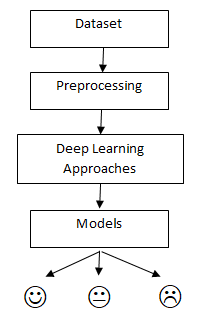
\includegraphics[scale=0.70]{../../../../../../../../umbalanced_paper/umb_class2021/images/baseline}}
		\caption{Methodology.}
		\label{fig}
	\end{figure}
	
	\subsubsection{Preprocessing}
	Because of the nature of writing on social media platforms, preprocessing is a critical operation. Its goal is to remove noise and words that are not properly written with alphabetical characters, as well as symbols such as Hashtags and URLs, among others. In this step, the use of Natural Language Processing is absolutely necessary. \\
	\subsubsection{Vector Representation}
	A vector representation is required to use Machine Learning algorithms, including deep learning in order to perform certain mathematical operations.  In the literature, a variety of strategies were utilized to attain this purpose, including:
	Bag of Words (BoW), Term Frequency-Inverse Document Frequency (Tf-IDF), and complicated representations that use semantics and context-named Word Embeddings like FastText, GloVe, and Word2Vec...
	\subsubsection{Deep Learning}	
Traditional machine learning models, such as support vector machine (SVM), logistic regression (LR), and so forth, require explicit features to be created, making it difficult to select the most important words that predominate the sentences or text. As a result, the accuracy of models varies between datsets. To solve this problem Deep learning approaches are required  because they apply automatic techniques to select features. Many approches are used in text classification, among them LSTM , BILSTM, GRU, CNN, and which gives an important accuracy in balanced datasets. However, in imbalanced datasets, all approaches produce low accuracy due to the overfitting problem caused by text features. This prompted us to include a module called Balancing in the baseline algorithm to address the issue as shown in Figure 2. 


\begin{figure}[htbp]
	\centerline{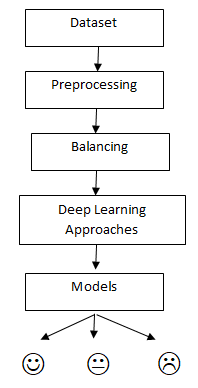
\includegraphics[scale=0.70]{../../../../../../../../umbalanced_paper/umb_class2021/images/balancing}}
	\caption{The new Baseline.}
	\label{fig}
\end{figure}

	\section{Balancing}
	In unbalanced datasets, certain classes have far more instances than others. Especially on social media platforms where neutral phrases predominate. As a result, deep learning model creation does not provide good accuracy.  There are three types of techniques that can be used to address this issue: Oversapling, Undersampling and Hybrid approach.\\
	\subsubsection{Undersampling}
	The undersampling is the process of increasing the number of samples from the minority class until a desired balancing ratio R reached which is  caculed with the Equation 1, while $X_{minority}$ is the minority class and $X_{majority}$ is the majority.
	\begin{equation}
	R(X)= \frac{X_{minority}}{X_{majority}}
	\end{equation}
	
	The aim is to create new samples from existing ones. There are two techniques for balancing with oversampling: random and synthetic.\\
	The first method is to collect random samples from the minority class and duplicate them until they reach a certain ratio when compared to the majority class. The problem with this method is that it is prone to overfitting due to the use of the same texts in balancing.We can reduce the possibility of overfitting by decreasing the ratio. \\
	
	The second technique, known as Synthetic Minority Over-Sampling Technique (SMOTE), generates samples through interpolation, which generates new data points within the range of known data points.
	The minority class is oversampled by creating synthetic samples rather than extracting data at random, which avoid duplication.\\
	
	\subsubsection{Oversampling}
	The oversampling method\textquotesingle s aim is to reduce the number of samples from the majority class. This approach have two principles Random, and Boundary.\\
	
	The first is a naive technique based on randomly removing samples until a desired ration R is reached. If R equals one, the class is perfectly balanced. The disadvantage of this method is that we can omit important details that can aid in the creation of a good model.\\
	
	The second technique extract samples at the boundary of two or more classes. it use an algorithm named Condensed Nearest Neighbours (CNN). The algorithm tends to select points near the boundary between the classes and transfer them to the new group. 
	
	\subsubsection{Hybrid Method}	
	The hybrid method combines the benefits of undersampling and oversampling, allowing us to amplify the minority class while removing any noisy observations. 
	
	
	\subsection{Results and Discussion:}\label{AA}
	
	
	\section{Conclusion}
	
	\bibliographystyle{IEEEtran}
	
	
	%\bibliography{IEEEabrv,../references/ref01}
	
\end{document}
